% This file provides an example Beamer presentation using the RWTH theme
% showcasing some of the more common options, similar to the Powerpoint version
% 12.11.2014: Revision 1 (Harold Bruintjes, Tim Lange)

% For RWTH, beamer should be loaded with class option t (top)
\documentclass[t]{beamer}

% Use fontspec to get Arial font
% Requires use of XeLaTeX
\usepackage{fontspec}
\setmainfont{Arial}
\setsansfont{Arial}
% Also force Arial for math for a more consistent look
\usepackage{unicode-math}

% https://tex.stackexchange.com/questions/426088/texlive-pretest-2018-beamer-and-subfig-collide
\makeatletter
\let\@@magyar@captionfix\relax
\makeatother

% German style date formatting (footer)
\usepackage[ddmmyyyy]{datetime}
\renewcommand{\dateseparator}{.}

\usepackage{MnSymbol,wasysym}

% Format the captions used for figures etc.
\usepackage[compatibility=false]{caption}
\captionsetup{singlelinecheck=off,justification=raggedleft,labelformat=empty,labelsep=none}

% PGFPlots is used for drawing some of the charts
\usepackage{pgfplots}
\pgfplotsset{compat=newest}
% This file contains some styles and macros for drawing charts similar to those of MS Office

\pgfplotsset{hor_barchart/.style={
  xbar=0mm,
  xmin=0,
  xtick=\empty,
  axis y line*=left,
  x axis line style={opacity=0},
  bar width=0.6cm,
  ytick=data,
  nodes near coords,
  every axis/.append style={font=\normalsize},
  every node near coord/.append style={font=\normalsize},
  nodes near coords align={horizontal},
  legend style={at={(0,-10mm)},anchor=north west,legend columns=-1,draw=none},
}}

\pgfplotsset{ver_barchart/.style={
  ybar=0mm,
  x = 4.5cm,
  ymin=0,
  ymajorgrids,
  axis x line*=bottom,
  y axis line style={opacity=0},
  bar width=0.8cm,
  enlarge x limits={0.15},
  xtick=data,
  nodes near coords,
  every axis/.append style={font=\normalsize},
  every node near coord/.append style={font=\normalsize},
  nodes near coords align={vertical},
  legend style={at={(0,-10mm)},anchor=north west,legend columns=-1,draw=none},
}}

\tikzstyle{chart}=[
    legend label/.style={font={\normalsize},anchor=west,align=left},
    legend box/.style={rectangle, draw=none, minimum size=5pt},
]

\tikzstyle{pie chart}=[
    chart,
    slice/.style={line cap=round, line join=round,draw=none},
    pie title/.style={font={\bf}},
    slice type/.style 2 args={
        ##1/.style={fill=##2},
        values of ##1/.style={}
    }
]

\newcommand{\pie}[3][]{
    \begin{scope}[#1]
    \pgfmathsetmacro{\curA}{90}
    \pgfmathsetmacro{\r}{1}
    \def\c{(0,0)}
    \node[pie title] at (90:1.3) {#2};
    \foreach \v/\s in{#3}{
        \pgfmathsetmacro{\deltaA}{\v/100*360}
        \pgfmathsetmacro{\nextA}{\curA + \deltaA}
        \pgfmathsetmacro{\midA}{(\curA+\nextA)/2}

        \path[slice,\s] \c
            -- +(\curA:\r)
            arc (\curA:\nextA:\r)
            -- cycle;

        %\begin{pgfonlayer}{foreground}
        % Position labels at 1.2 times radius (just outside of chart)
        \path \c -- node[pos=1.2,pie values,values of \s]{$\v\%$} +(\midA:\r);
        %\end{pgfonlayer}

        \global\let\curA\nextA
    }
    \end{scope}
}

% Custom legend (used for pie chart)
\newcommand{\legend}[2][]{
\begin{scope}[#1]
  \path
    \foreach \n/\s in {#2} {
      ++(0,-5pt) node[\s,legend box] {} +(5pt,0) node[legend label] {\n}
    };
\end{scope}
}


% Load the actual RWTH theme. Suggested is to load the full theme,
% as it requires some specific dimensions
\usetheme{rwth}

% -------------------- My Packages -------------------- %
\usepackage{hyperref}
\usepackage{xcolor}
\usepackage[utf8]{inputenc}

% \usepackage{fontspec}
\setmonofont{Roboto Mono}
\usepackage{minted}
\newcommand\pycode[1]{\inputminted[frame=lines, framesep=2mm, fontsize=\normalsize]{python}{#1}}

\definecolor{comment}{HTML}{aaaaaa} % italic
\definecolor{string}{HTML}{448c27}


%---------- Ich bin ein verdammter Künstler ----------
\usepackage{listings}
\definecolor{maroon}{RGB}{128, 0, 0}
\definecolor{pinegreen}{RGB}{1, 121, 111}
\definecolor{darkmidnightblue}{RGB}{0, 51, 102}
\definecolor{rwthblue}{RGB}{0, 84, 159}
% www.colorhexa.com for color references

% ---------- Hyperref -----------
\hypersetup{colorlinks=true,
            breaklinks=true,
            urlcolor=rwthblue,
            linkcolor=rwthblue,
            citecolor=rwthblue}
\def\UrlBreaks{\do\/\do-}
% -------------------------------


\begin{document}
\logo{
\includegraphics{logo.png}}

% Setup presentation information
\title{Back-Propagation and Algorithms for Training Artificial Neural Networks with TensorFlow}
\date{10. Dezember 2020}
\author{Gero Kauerauf}

\frame{\titlepage}

\section{Überblick}
% Frame with items
\begin{frame}
    \begin{itemize}
        \item Bildklassifizierung mit TensorFlow.Keras
        \begin{itemize}
            \item Was soll unser Modell können?
            \item Unser Datensatz
            \item Konstruktion unseres Python-Programms
        \end{itemize}
    \end{itemize}
\end{frame}

\section{Was soll unser Modell können?}
\begin{frame}
    \begin{itemize}
        \item Wir möchten ein Modell, welches unterschiedliche Blumen erkennen kann
        \item Wir haben eine Sammlung an von Menschen klassifizierten Bildern von Blumen
        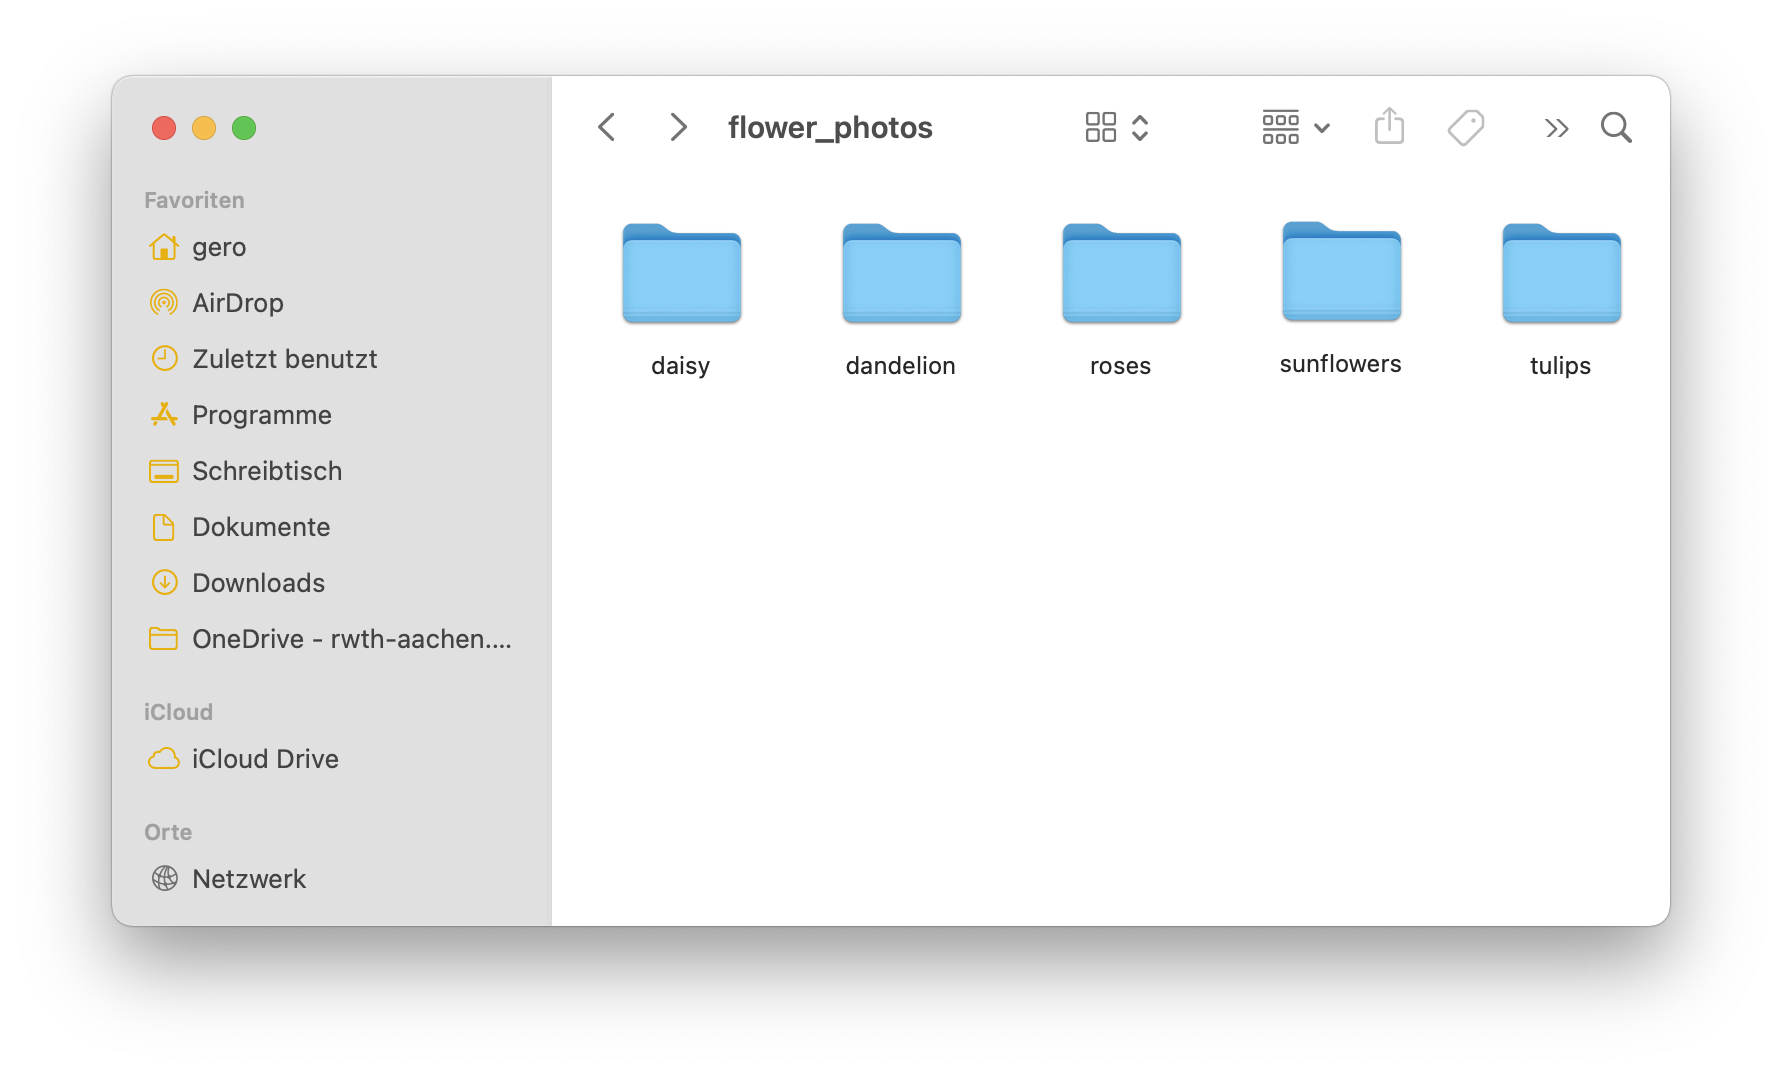
\includegraphics[width=0.5\textwidth]{teach-plots/flower-photos}
        \item Enthalten sind Bilder von Gänseblümchen, Löwenzahn, Rosen, Sonnenblumen und Tuplen
        \item Mit diesem Datensatz können wir ein Modell bauen, welches zwischen genau diesen unterscheiden kann
    \end{itemize}
\end{frame}

\section{Datensatz}
\begin{frame}
    \begin{itemize}
        \item Hier ein kleiner Einblick in unseren Datensatz
    \end{itemize}
    \begin{figure}
        \centering
        \begin{minipage}{0.4\textwidth}
            \centering
            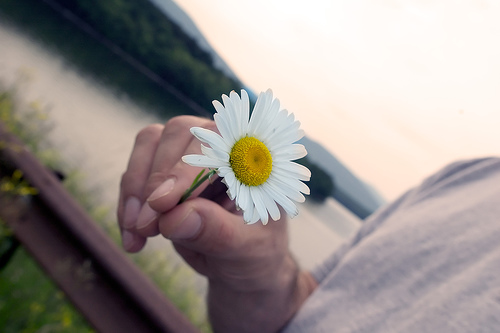
\includegraphics[width=0.8\textwidth]{./teach-plots/dandelion.jpg} % first figure itself
        \end{minipage}\hfill
        \begin{minipage}{0.4\textwidth}
            \centering
            
\includegraphics[width=0.5\textwidth]{./teach-plots/rose.jpg} % second figure itself
        \end{minipage}
    \end{figure}
    \begin{figure}
        \centering
        \begin{minipage}{0.4\textwidth}
            \centering
            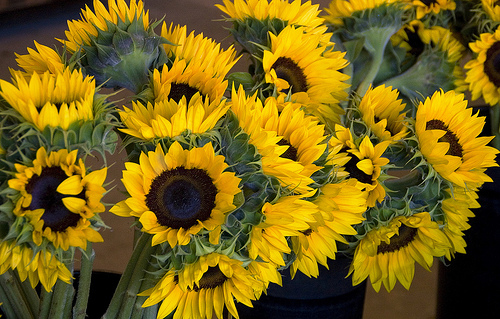
\includegraphics[width=0.8\textwidth]{./teach-plots/sunflower.jpg} % first figure itself
        \end{minipage}\hfill
        \begin{minipage}{0.4\textwidth}
            \centering
            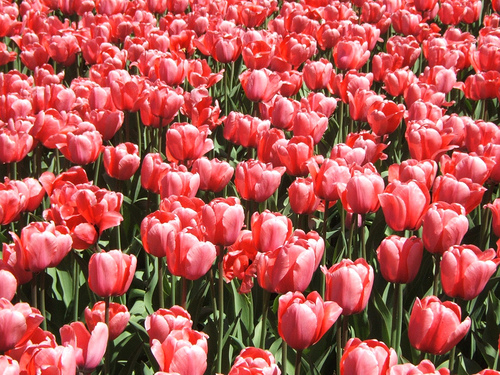
\includegraphics[width=0.68\textwidth]{./teach-plots/tulip.jpg} % second figure itself
        \end{minipage}
    \end{figure}
\end{frame}

\section{Datensatz}
\begin{frame}
    \begin{itemize}
        \item Zuerst wollen wir unseren Datensatz laden
        \item Dazu definieren wir zuerst die Bildgrößen und die Batch-size
        \pycode{./code-snippets/dataset-params.py}
        \item Danach möchten wir unseren gesammten Datensatz in einen Trainings- und einen Validierungssatz aufteilen
        \item Mit dem Trainingssatz werden wir dann tatsächlich unser MLP trainieren
        \item Den Validierungssatz nutzen wir um unser Modell nach dem Training beurteilen zu können.
    \end{itemize}
\end{frame}

\section{Datensatz}
\begin{frame}
    \begin{itemize}
        \item Dazu nutzen wir die Methode \texttt{image\_dataset\_from\_directory} aus \texttt{tf.keras.preprocessing}
        \pycode{./code-snippets/dataset-from-directory.py}
    \end{itemize}
\end{frame}

\section{Leistungsoptimierung}
\begin{frame}
    \begin{itemize}
        \item Wir werden nun zwei Methoden verwenden um das Laden der Daten beim Training zuverbessern
        \item \texttt{Dataset.cache()}
        \begin{itemize}
            \item Geladene Bilder werden im RAM gelassen und nicht jedes mal erneut eingeladen
        \end{itemize}
        \item \texttt{Dataset.prefetch()}
        \begin{itemize}
            \item Datenvorverarbeitung und Modelltraining werden überlappt
            \item Im \(i\)-ten Trainingsschritt werden die Daten für den den \(i+1\)-ten Schritt gelesen.
        \end{itemize}
    \end{itemize}
\end{frame}

\section{Leistungsoptimierung}
\begin{frame}
    \begin{itemize}
        \item Ohne prefetching
    \end{itemize}
    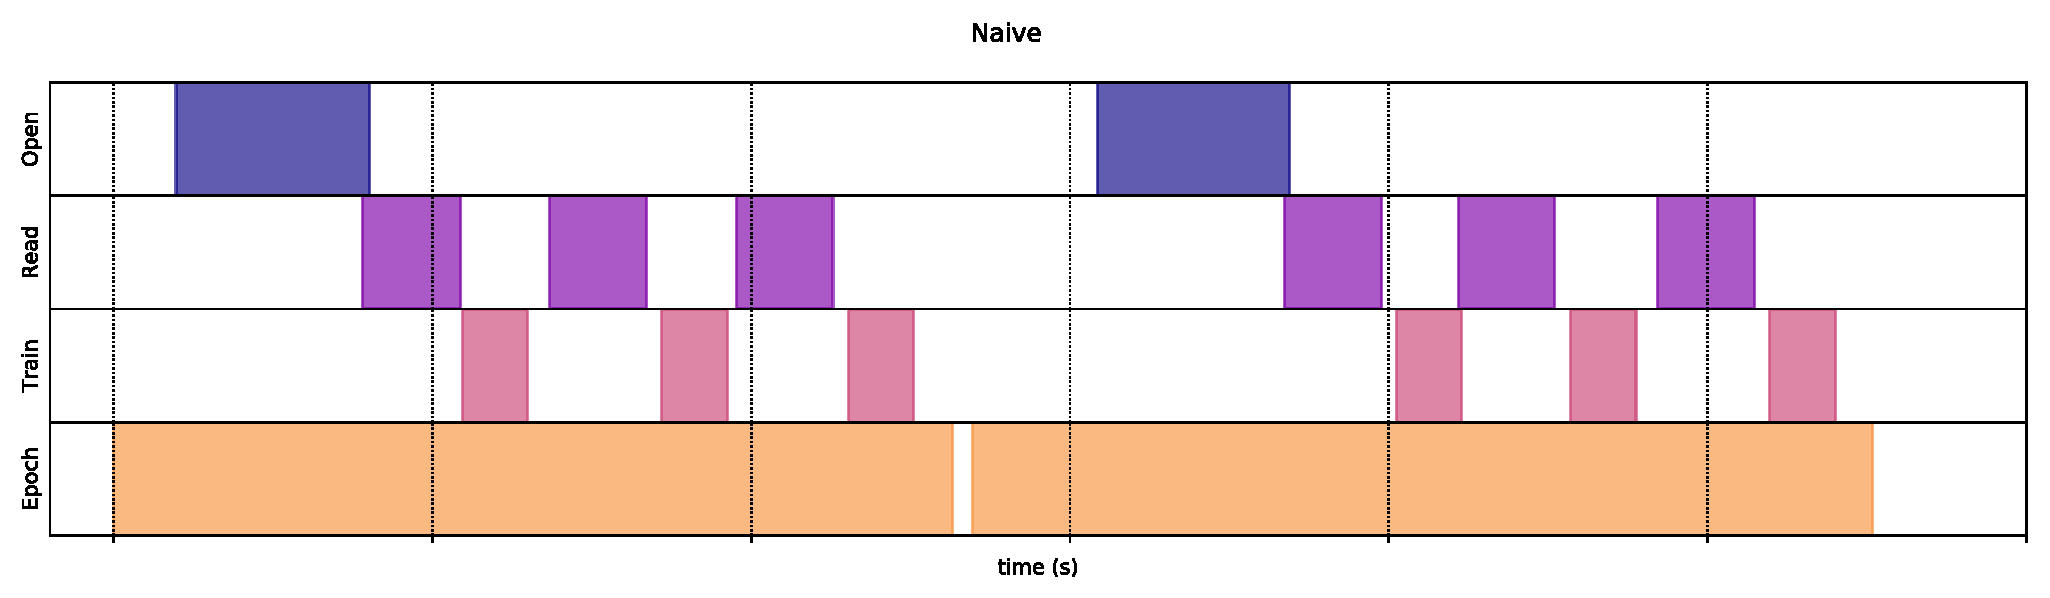
\includegraphics[width=0.7\textwidth]{teach-plots/naive-prefetching-crop.pdf}
    \begin{itemize}
        \item Mit prefetching
    \end{itemize}
    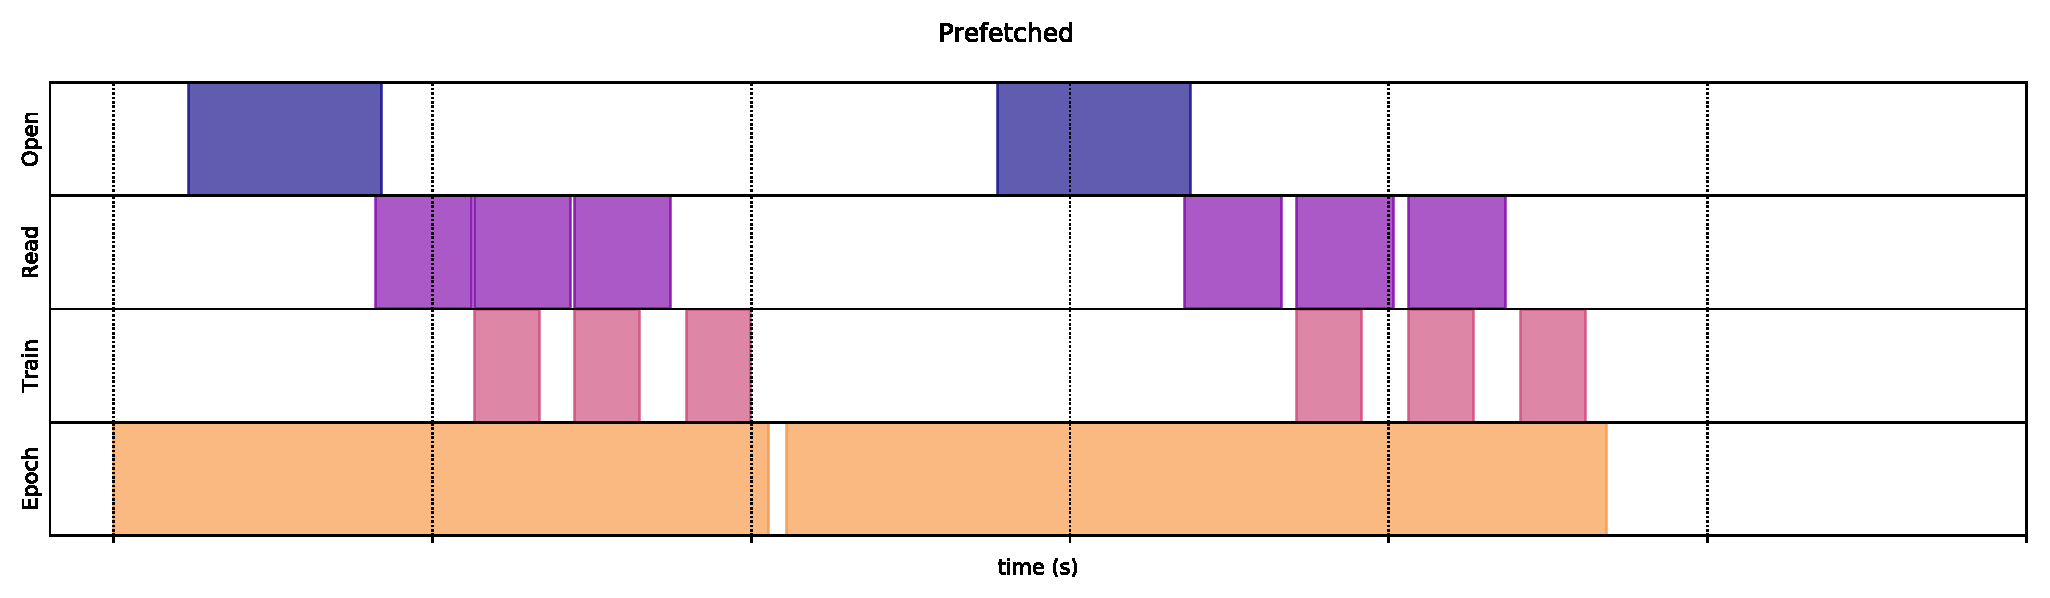
\includegraphics[width=0.7\textwidth]{teach-plots/prefetched-crop.pdf}
    \large\href{https://www.tensorflow.org/guide/data_performance}{https://www.tensorflow.org/guide/data\_performance}
\end{frame}

\section{Leistungsoptimierung}
\begin{frame}
    \begin{itemize}
        \item Außerdem nutzen wir noch die experimentelle Methode \texttt{AUTOTUNE}
        \item Diese kann die \texttt{buffer\_size} von \texttt{prefetch} dynamisch zur Laufzeit anpassen
        \pycode{./code-snippets/dataset-optimize.py}
    \end{itemize}
\end{frame}

\end{document}
